% !TEX root = template.tex

\section{Results}
\label{sec:results}

%In this section, you should provide the numerical results. You are free to decide the structure of this section. As a general ``rule of thumb'', use plots to describe your results, showing, e.g., precision, recall and \mbox{F-measure} as a function of the system (learning) parameters. You can also show the precision matrix. 


The results obtained with these models are shown in Table \ref{table:results}, which also shows the 95\% confidence intervals from tree  different trials.

\begin{table}
	\centering
	\begin{tabular}{|l|l|l|l|}
    \hline
    model  & parameters & accuracy  & time \\
    \hline
    res3 & 20,380 & 0.8445 & 5849ms \\
    \hline
    res6 & 40,330 & 0.8560 & 7384ms\\
    \hline
    res9 & 60,280 & 0 & 0 \\
    \hline
    vit10x10 & 42,756 & 0 & 0  \\
    \hline
    vit10x8  & 54,044 & 0 & 0  \\
    \hline
    vit20x10  & 26,284 & 0.7597 & 3242ms \\
    \hline
    \end{tabular} 
\label{table:results}
\caption{Results obtained per each model over 3 trials}
\end{table}

\begin{figure}[h]
    \centering
    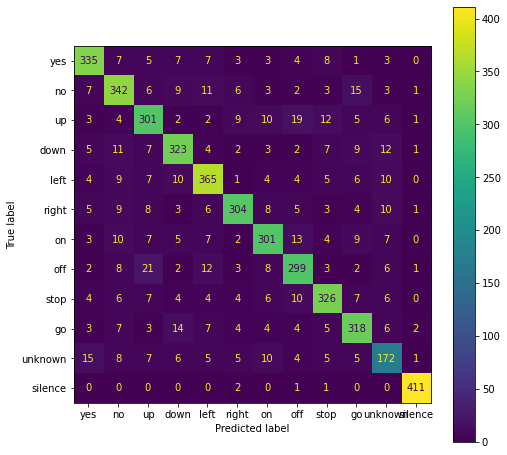
\includegraphics[width=0.5\textwidth]{confusion_matrix_res3_keyword.png}
    \label{fig:confusionmatrix}
    \caption{Confusion Matrix of the model res3}
\end{figure}


Checking the confusion matrix of model res3 \ref{fig:confusionmatrix}, we can observe well the accuracy is no so high. We can notice that the best label that the model predicts is unknown, and also we can observe that the model sometimes doesn't predict well for labels off and up.  

%
%\begin{remark}
%Present the material in a progressive and logical manner, starting with simple things and adding details and explaining more complex findings as you go. Also, do not try to explain/show multiple concepts within the same sentence. Try to \textbf{address one concept at a time}, explain it properly, and only then move on to the next one.
%\end{remark}
%
%\begin{remark}
%The best results are obtained by generating the graphs using a vector type file, commonly, either \texttt{encapsulated postscript (eps)} or \texttt{pdf} formats. To plot your figures, use the Latex \texttt{\textbackslash includegraphics} command. Lately, I tend to use pdf more.
%\end{remark}
%
%\begin{remark}
%If your model has hyper-parameters, show selected results for several values of these. Usually, tables are a good approach to concisely visualize the performance as hyper-parameters change. It is also good to show the results for different flavors of the learning architecture, i.e., how architectural choices affect the overall performance. An example is the use of CNN only or CNN+RNN, or using inception for CNNs, dropout for better generalization or attention models. So you may obtain different models that solve the same problem, e.g., CNN, CNN+RNN, CNN+inception, etc.
%\end{remark}
